\documentclass[11pt]{article}
%\documentclass[12pt]{article}
\usepackage[margin=1.25in]{geometry} 
\usepackage{amsmath}
\usepackage{tcolorbox}
\usepackage{amssymb}
\usepackage{amsthm}
\usepackage{lastpage}
\usepackage{fancyhdr}
\usepackage{accents}
\usepackage{listings}
\pagestyle{fancy}
\setlength{\headheight}{40pt}

\newenvironment{solution}
  {\renewcommand\qedsymbol{$\blacksquare$}
  \begin{proof}[Solution]}
  {\end{proof}}
\renewcommand\qedsymbol{$\blacksquare$}

\newcommand{\ubar}[1]{\underaccent{\bar}{#1}}
\usepackage[utf8]{inputenc}
\usepackage{graphicx}
\usepackage{biblatex}
\usepackage{xurl}
\usepackage{hyperref}
\hypersetup{urlcolor=blue}

\bibliography{ref}

\begin{document}
\begin{titlepage}

\newcommand{\HRule}{\rule{\linewidth}{0.5mm}} % Defines a new command for the horizontal lines, change thickness here

\center % Center everything on the page
 
%----------------------------------------------------------------------------------------
%	HEADING SECTIONS
%----------------------------------------------------------------------------------------

\textsc{\LARGE \bf A Novel Approach to Protein-Protein Interaction 
Network Analysis via Modern Computational 
Methodologies}\\[1.0cm] % Your Project Title
\textsc{\large Kaavish Project Proposal}\\[0.5cm]
\textsc{\large By}\\[0.5cm] 

%----------------------------------------------------------------------------------------
%	AUTHOR SECTION
%----------------------------------------------------------------------------------------

\begin{minipage}{0.8\textwidth} % Type Team Members Details here
\begin{center} \large
Ali \textsc{Hamza} 05084 (\href{mailto:ah05084@st.habib.edu.pk}{\texttt{ah05084@st.habib.edu.pk}}) \\
Haris Karim \textsc{Ladhani} 04349 (\href{mailto:hl04349@st.habib.edu.pk}{\texttt{hl04349@st.habib.edu.pk}})\\
Maham Shoaib \textsc{Patel} 04911 \href{mailto: (mp04911@st.habib.edu.pk)}{(\texttt{mp04911@st.habib.edu.pk})}\\
Muhammad Usaid \textsc{Rehman} 04302 (\href{mailto:mr04302@st.habib.edu.pk}{\texttt{mr04302@st.habib.edu.pk}}) \\
\end{center}
\end{minipage}
~
\begin{minipage}{0.4\textwidth}
%\begin{flushright} \large
%\emph{Supervisor:} \\
%Dr. James \textsc{Smith} % Supervisor's Name
%\end{flushright}
\end{minipage}\\[1cm]

% If you don't want a supervisor, uncomment the two lines below and remove the section above
%\Large \emph{Author:}\\
%John \textsc{Smith}\\[3cm] % Your name

%----------------------------------------------------------------------------------------
%	DATE SECTION
%----------------------------------------------------------------------------------------

{\large \today}\\[1cm] % Date, change the \today to a set date if you want to be precise

%----------------------------------------------------------------------------------------
%	LOGO SECTION
%----------------------------------------------------------------------------------------


\includegraphics[height=5cm]{HU_logo_new.png}\\[0.5cm] % Include a department/university logo - this will require the graphicx package
 
%----------------------------------------------------------------------------------------
\begin{minipage}{0.8\textwidth}
\begin{center} \large
In partial fulfillment of the requirement for \\
Bachelor of Science \\
Computer Science \\
\end{center}
\end{minipage}\\[1cm]

\textsc{\large Dhanani School of Science and Engineering}\\[0.5cm]
\textsc{\large Habib University}\\[0.5cm] 
\textsc{\large Fall 2021}\\[0.5cm] 

\begin{minipage}{0.8\textwidth}
\begin{center} \large
Copyright~\textcopyright~2021 Habib University
\end{center}
\end{minipage}

\vfill % Fill the rest of the page with whitespace

\end{titlepage}

\lhead{Habib University \\ Kaavish Project Proposal Report } 
\rhead{A Novel Approach to Protein-Protein Interaction Network \\ Analysis Via Modern Computational Methodologies \\ Fall 2021} 
\rfoot{Team \textsc{Prions}}
\cfoot{\thepage\ of \pageref{LastPage}}

%\maketitle

\section{Problem Definition}
\label{lblPD}

    \subsection{Background}
    The number of all known proteins remains unknown but we have an ever growing database that is currently reaching almost a 100,000 unique molecules. It is estimated that a single human cell holds 42 million protein molecules. (It should be noted that these figures are not exact and are only estimates as they have been acquired through rigorous experimental study.)
    
    Furthermore, the number only holds relevance to humans which speeds to vastness of proteins in the known world. Therefore, the study of protein-protein interactions is of great importance and warrants a thorough investigation. Current experimental limitations result in the field leaning on computational methods to attempt to study the problem. The computational methods are not yet fully developed and the results are not yet satisfactory which is why our project aims to attempt to develop a novel computational method, using present methods in congregation with some newer techniques to attack the weaknesses present in present methods, to attempt to study the problem with further accuracy and speed. 
    
    A protein is said to be made up of chemical building blocks known as Amino Acids. A protein chain is essentially a list of such amino acid molecules. This chain is known as a primary protein structure. The arrangement of these molecules dictates the nature of the protein. The primary protein can then fold to create a secondary protein molecule, where, once again, the folding of the protein establishes its nature. The secondary protein can further fold to create a tertiary protein structure. Finally, these tertiary protein molecules, also known as macro molecules form to create a quaternary protein structure, and the way two macromolecules interact influences the nature of the resulting protein. The interaction of these protein often plays an important role in understanding drug-making, and various other biological processes and thus makes the subject and important area of study.
    
    \begin{figure}[h!]
        \centering
        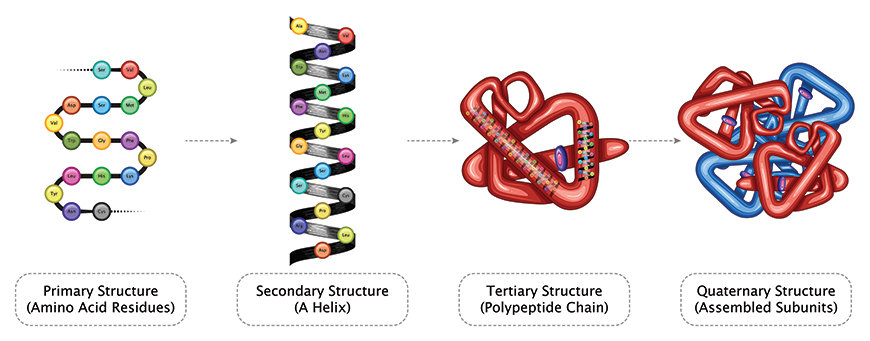
\includegraphics[scale = 0.45]{Proposal/images/PROTEINS-2.jpg}
        \caption{4 Stages of a Protein Structure}
        \label{fig:proteindef}
    \end{figure}
    
    \newpage
    
    One method to understand protein-protein interactions is through the use of networks. PPI networks are constructed from PPI data sets by denoting proteins as nodes and PPIs as edges. Usually, PPI networks are static, such that that it is assumed that PPI is constant in all cells, and .conditions. However, real PPI are dependent on various factors such as spatial, temporal, and contextual variations and thus may be represented better through Dynamic PPI networks. Furthermore, to study cross-specie PPI interlog PPI networks are also being utilized to where each node may represent a protein complex. 
    
    The computational methods applied to these networks aim to detect meaningful clusters from PPI networks as protein complexes based and are largely of three categories:
    \begin{enumerate}
        \item Cluster-quality based methods
        \item Node-affinity based methods
        \item Ensemble clustering methods.
    \end{enumerate}
    The results of these methods are then judged on various metrics, of which, the following 6 are quite common:
    \begin{enumerate}
        \item Precision, Recall
        \item F-measure
        \item Sensitivity (Sn)
        \item Positive Predictive Value (PPV)
        \item Positive Predictive Value (PPV)
        \item Accuracy (Acc) 6
        \item Proportion of Significant Complexes (PSC).
    \end{enumerate}
    \subsection{Problem Statement}
    
    The protein-protein interaction (PPI) is a vastly studied area and thus there are various datasets and computational methods available to tackle the issue but these are far from perfect. Not only are the datasets incomplete (they cover less than 60\% of non-redundant human PPI), the prediction models are also lacking in completely capturing the notion of a PPI. This leads to a very interesting space for us to attempt to innovate. Thus the problem can be broken down into three parts:
    
    \begin{enumerate}
        \item Datasets are (1) Incomplete, and (2) contain false-positivies.
        \item PPI networks are represented statically, instead of dynamically.
        \item Protein Complex identification methods do not account for various factors such as (1) real protein complexes being small and sparse, and (2) using network topological features instead biological data for scoring. 
    \end{enumerate}
    
    These issues can be addressed through various methods, and our research directs us towards using: 
    \begin{enumerate}
        \item An approach to work with dynamic PPI networks to account for various missing factors that static PPI networks overlook.
        \item Use of generative models to adjust for the incomplete datasets
        \item Use of ensemble clustering methods to adjust for various differences in protien complexes
    \end{enumerate}
    
    % 1. Lacking in present PPI datasets -> Leads to Unreliable performance of Present Models -> Potential Solution is to use Generative Network Models, and integrating further biological information may create better datasets
    
    % 2. 3 Types of PPI networks are present: Static, Dynamic, and Interlog Networks
        
        % "PPI networks are constructed from PPI data sets by     denoting
        % proteins as nodes and PPIs as edges. Typically, PPI networks are
        % static, assuming every PPI is constant in any cell and condition.
        % However, PPIs are dynamic inside cells, and their occurrences
        % depend on spatial, temporal and/or contextual variation. Therefore,
        % it is more reasonable to model PPI networks as dynamic
        % systems" [71] Besides, as more and more PPI data from different
        % species are available, constructing interolog PPI networks
        % becomes a new trend to transfer biological knowledge across
        % species [72].
        
    % However, most of the protein complex features are network             topological features, preventing the performance improvement of      these models. Therefore, biologically relevant protein complex        features should be explored to improve the performance of the          supervised models.

    %3. Computational Methods
        % Computational methods detect meaningful clusters from PPI
        % networks as protein complexes. According to their method
        % ologies, these methods can be organized into three categories, including cluster-quality-based methods, node-affinity-based methods and ensemble clustering methods.
    
    %4. Evaluation Metrics
    % Seven metrics are commonly used for evaluating protein
    % complex identification methods, including Precision, Recall,
    % F-measure, Sensitivity (Sn), Positive Predictive Value (PPV),
    % Accuracy (Acc), and Proportion of Significant Complexes (PSC).
    
    
    
    
\section{Project Relevance to Society}
\label{lblPRS}
% $<$explain, how your project addressing some societal/real-world problem?$>$
Protein-Protein Interaction (PPI) alongside other
molecular interactions play an integral role in
essential biological functions such as transport
of substances, gene expression control, enzyme
inhibition etc. Protein complexes formed through
these PPI networks are responsible for their own
biological functions. Studying and identifying
these protein complexes and corresponding PPI
networks that form these complexes allows us to
further our understanding of functions and
organizations of cells. 

Multiple experimental techniques have been
designed over recent years to identify protein complexes from cells such as NMR, X-ray crystallography or the most popular; tandem
affinity purification with mass
spectrometry (TAP-MS). The problem with these
identification techniques is they are quite
difficult to perform along with being
significantly more expensive than their
computational counterparts. Additionally, the
TAP-MS method is notoriously known to often
produce incomplete and unreliable results due to
the presence of technical biases.

To counter the problems faced in conducting
biological experimental techniques, several
powerful computational methods have been
developed to discern and identify protein
complexes from PPI networks. These PPI networks
are stored in several biological databases such as DIP and have been validated by biological experiments.

The existing computational methods such as
ClusterONE and Core\&Peel are known for their
performance within the field but they still are
not entirely precise with their predictions of
protein complexes and can only identify large and
dense protein complexes. We aim to target this
particular limitation of the current
computational methods by identifying smaller and
sparse protein complexes as are actually found in
real life. 

\section{Originality/Novelty}
\label{lblNov}
% $<$ Is the problem worth-solving? What other solutions exists? What is the novelty of your project?$>$
% present methods -> cluster quality methods -> local clusters, global clusters 
% local clustering: NCMine, Core&Peel, TP-WDPIN, DME
% global-cluster-quality-based methods: RNSC, MAE-FMD, LCMA, SGNMF
% PPSampler (Monte Carlo Methods)

% Node affinity based methods, local-node-affinity-based-methods
% global-node-affinity-based-methods

% Ensemble clustering 
% 17 different algos analyzed 
% problems: - small and sparse protein complexes not identified
%           - some proteins can only be identified by one method -> confidence score
%           - some algos have p bad accuracy

% approach: - meta-predictor using more biological info
%           - give unique proteins high confidence scores
%           - take care of false complexes
%           - ensemble methods -> multiple methods working in conjunction
%           - generative network models -> solve PPI data-set issues
% explore supervised machine learning methods in this context combined with increased 
% biological data
% 
Protein complexes within protein-protein interaction (PPI) networks have essential roles 
in regulatory processes and cellular functions. Protein complexes have also been viable candidates 
in cancer treatment research. %(cite https://doi.org/10.1016/B978-0-12-417150-3.00015-6)%
Therefore protein complex identification is an important problem that has a lot of unexplored
potential. 

Protein complex identification has been a widely researched problem in computational biology. 
Identifying protein complexes using experimental methods often ends up disrupting the behavior and 
structure of the complex, which means that computational methods are better suited for this task. 
There are several computational methods that exist to predict protein complexes within PPI networks
that employ various techniques such as cluster quality (local and global clustering) and node affinity 
based methods. A newer approach is to use ensemble clustering methods which combine 
different clustering methods into one meta-predictor. 

There are approximately 17 pre-existing different algorithms/meta-predictors that predict/identify protein complexes. However, 
these are far from perfect. Small and sparse protein complexes are ignored by these predictors. 
Moreover, several protein complexes can only be detected by a single existing algorithm which means that 
meta-predictors can often ignore these protein complexes due to low confidence scores. 

The performance of these algorithms is quite varied. On the DIP dataset, the best accuracy that was 
obtained was around 62\% using the \textsc{CFinder} method and the \textsc{MCode} method, both local-node-affinity 
methods. In other data sets, the SPiCi database and CMC method also performed well 
and reached an accuracy of about 80\%. 

We will be developing a novel method in an attempt to improve the accuracy of preexisting models. Our
planned meta-predictor will attempt to incorporate more biological data compared to preexisting
meta-predictors. We will also attempt to incorporate statistically accurate predictions of 
unique proteins while also considering predictions of false complexes. We will be using a collection 
of preexisting models combined in order to construct the meta-predictor. 
Our work will also include a generative network model such as GAN which can potentially 
contribute in fixing the incompleteness and unreliability of protein-protein interaction data sets.


\section{CS Contribution}
\label{lblCSCont}
% $<$Does it have significant CS contribution? Which higher level CS courses contribute to this?$>$
Bioinformatics is an incredibly vast field that encapsulates a multitude of different areas. Protein-protein
interactions and protein complexes have been widely studied in the past and there is a significant amount 
of preexisting literature. We will build on preexisting tools and ideas to attempt to create novel methods that
aim to improve the accuracy of preexisting models. The computer science courses we will apply are:
\begin{itemize}
    \item Computational Intelligence: This will help us experiment with
    different optimization methods in order to obtain a better predictor. 
    \item Graph Theory: Since protein networks are represented as graphs, we will apply our knowledge of 
    graphs in this project.
    \item Introduction to Computational Social Science: We will be using the networks part of the course 
    in understanding PPI networks.
    \item Deep Learning: We will be using deep learning as well as machine learning to potentially create
    our predictor.
    \item Computer Graphics: This will be used in visualizing the real-time visualizer component of our 
    Kaavish.
    \item Probability \& Statistics: This will provide us with the necessary mathematical background 
    for our prediction model.
\end{itemize}

\section{Scope and Deliverables}
\label{lblScope}
The deliverables and scopes that are mentioned below are subject to minor changes as the project keeps 
developing due to unforeseen events or situations. However, the Kaavish committee will be informed in such 
cases and it would be made sure that the deadlines set by the committee are not compromised. Below is a 
concatenation of the deadlines set by the committee and the potential deadlines for the deliverables set by 
the team.

\begin{center}
\begin{tabular}{|l|l|}
\hline
 \textbf{Deliverable} & \textbf{Expected Time}  \\
 \hline \hline
 Literature Review & Early November\\
 Software Requirements Specification (SRS) &  5 November, 2021\\
 Software Design Specification (SDS) &  30 November, 2021  \\
 Dataset Compilation \& Creation &  Early December  \\
 Initial Prediction Model &  Early December  \\
 Kaavish I Update &  8 December, 2021  \\
 Finalised Prediction Model &  Early February  \\
 Kaavish II - Midsemester Update &  22 March, 2022  \\
 Real-Time Visualizer &  Late March  \\
 Final Thesis &  Early May  \\
\hline
\end{tabular}
\end{center}

\section{Feasibility}
\label{lblFes}
\begin{itemize}
  \item \textbf{Data Sets} 
  
  There are several datasets available catering 
  to the research of protein-protein interaction networks. We list some of them below:
    \begin{table}[htpb]
      \centering
      \caption{A list of PPI databases.}
      \vspace{1 em}
      \label{tab:dataset1}
      \begin{tabular}{l|l}
      \hline
      Name & Website \\
      \hline
      DIP & \url{http://dip.doe-mbi.ucla.edu/dip/Main.cgi}\\
      BioGRID & \url{https://thebiogrid.org/} \\  
      HPRD & \url{http://www.hprd.org/} \\ 
      MINT & \url{https://mint.bio.uniroma2.it}\\
    STRING & \url{https://string-db.org/} \\
    \hline
    \end{tabular}
  \end{table}

  \begin{table}[h]
    \centering
    \caption{A list of protein complex databases.}
    \vspace{1 em}
    \label{tab:dataset2}
    \begin{tabular}{l|l}
    \hline
    Name  & Website \\
    \hline
    CYGD & \url{http://mips.gsf.de/genre/proj/yeast} \\
    CORUM & \url{http://mips.helmholtz-muenchen.de/corum}\\
    CYC2008 & \url{http://wodaklab.org/cyc2008} \\
    PISA & \url{http://www.ebi.ac.uk/msd-srv/prot_int/pistart.html} \\
    \hline
    \end{tabular}
  \end{table}
  \newpage
    \item \textbf{Hardware}\vspace{0.25em}
    
    We are going to be working on extensive neural networks and will require immense computational power. Hence, we will be making use of GPUs for parallel computation or a virtual GPU environment in order to optimize computationally demanding algorithms within our solution. We will also make use of Google Colab for those members who do not have access to GPUs or when working on AI based implementations. 
    \item \textbf{Libraries}\vspace{0.25em}
    
    Our final solution to the problem is likely to make use of ML/DL techniques therefore the use of libraries such 
    as Tensorflows, Sklearn, etc will become imperative. Additionally,  will also be using matplotlib, pandas, and numpy to visualize and 
    analyze data. We will also explore other languages that are optimized for ML and data science such as Julia.
    \item \textbf{Challenges}
    
    Our core challenges as well as their predicted solutions can be listed down below as follows:
    \begin{enumerate}
        \item \textbf{A partially developed understanding of underlying biological processes}\vspace{0.25em} 
        Although the group has a core understanding of how protein complexes form and the processes revolving protein-protein interaction, a deeper and more thorough understanding of the topic is required to begin theorizing a concrete solution for the problem. We plan to continue to read various research papers, and consult various field experts as we have so far in order to account for this shortcoming.
        
        \item \textbf{Vast research in present methods} \vspace{0.25em}
        
        There is a lot of work that has been done in this area and this has resulted in a plethora of methods, in which few are very efficient, thus it becomes a challenge for us to understand which methods must be considered and which should not and this warrants further research. 
        
        \item \textbf{Further research could offset the present plan} \vspace{0.25em}
        
        Our current research has provided us with a path that shows promise in being of value to the present research but due to the above stated challenges, this path could be offset if we find a better approach thus our group must always be prepared to spend more time on the FYP in case such a situation arises. 
        
    \end{enumerate}
\end{itemize}
% $<$Are the resources(datasets, computing, libraries, hardware) required to do the project available?$>$ 
% Datasets: list datasets from paper

% Hardware: GPU for parallel computation
% Libraries: 

\newpage
\section{Team Dynamics}
\label{lblTeam}
% $<$Does the team have capacity to address the problem? Have they taken relevant courses?$>$

Almost all members have taken courses in the relevant areas to some degree. 
Each member also has their own area of expertise which they will be 
employing to contribute meaningfully to the project.
\begin{enumerate}
    \item Ali Hamza
    \begin{enumerate}
        \item Relevant Courses: CS/MATH 326/320, IS/CS413, CS/SDP 262, CS 440, CS 201, CS 412, MATH 205, MATH 310
        \item Strengths: CS Theory, Mathematics, Research, Programming
        \item Weaknesses: Debugging, Technical Writing, Genetic Algorithms
    \end{enumerate} 
    \item Haris Karim Ladhani,
    \begin{enumerate}
        \item Relevant Courses: BIO 101, BIO 201, CS/SDP 262, MATH 205, CS 201, CS 353, EE 354, CS 355
        \item Strengths: Literature Research, Software Development, Agent Based Modeling, Technical Writing 
        \item Weaknesses: Intensive Programming, Algorithm Writing, Mathematical Analysis
    \end{enumerate} 
    \item Muhammad Usaid Rehman
    \begin{enumerate}
        \item Relevant Courses: CS 451, CS 412, IS/CS 413, CS 440, MATH 205, MATH 310, CS/SDP 262
        CS 201, CS 223
        \item Strengths: Research \& Literature Review, Programming,
        Statistics \& Mathematical Analysis, Design and Analysis of 
        Algorithms, Deep Learning, Genetic Algorithms
        \item Weaknesses: Data Mining, Debugging, Parallel Programming 
    \end{enumerate} 
    \item Maham Shoaib Patel
    \begin{enumerate}
        \item Relevant Courses: BIO 101, BIO 102, CS 375, CS 451, CS 412, CS 201, MATH 205, MATH 310
        \item Strengths: Literature Research, Programming, Genetic Algorithms, Parallel Programming
        \item Weaknesses: Mathematical Analysis, Technical Writing, CS Theory
    \end{enumerate} 
\end{enumerate}
\section{Internal Supervisor}
\label{lblIntSup}
\begin{enumerate}
    \item Dr. Waqar Saleem
    \item Dr. Saleha Raza
\end{enumerate}

\section{External Supervisor}
\label{lblExtSup}
    
    We have a potential external advisor, \href{https://www.researchgate.net/profile/Saeeda-Baig}{Dr. Saeeda Baig}

\nocite{*}
\printbibliography




\end{document}
